%!TEX TS-program = xelatex  
%!TEX encoding = UTF-8 Unicode  
      
\documentclass[a4paper, 11pt]{article}
\usepackage[top=1.5in, bottom=1.5in, left=1.0in, right=1.0in]{geometry} 
\usepackage{indentfirst}        
\usepackage{float}
\usepackage{amsmath}
\usepackage{hyperref}
\usepackage{graphicx}


\title{ARMA-GARCH}
\author{SHIHENG SHEN}
\date{\today}
\begin{document}
\maketitle

\section{Data}
\subsection{Data Source}
HadCRUT4 is a gridded dataset of global historical surface temperature anomalies relative to a 1961-1990 reference period. Data are available for each month since January 1850, on a 5 degree grid. The dataset is a collaborative product of the Met Office Hadley Centre and the Climatic Research Unit at the University of East Anglia. \\ $url = $\url{http://www.metoffice.gov.uk/hadobs/hadcrut4/data/current/time_series/HadCRUT.4.5.0.0.monthly_ns_avg.txt}.
\subsection{Brief Data Description}
The gridded data are a blend of the CRUTEM4 land-surface air temperature dataset and the HadSST3 sea-surface temperature (SST) dataset. The dataset is presented as an ensemble of 100 dataset realisations that sample the distribution of uncertainty in the global temperature record given current understanding of non-climatic factors affecting near-surface temperature observations. This ensemble approach allows characterisation of spatially and temporally correlated uncertainty structure in the gridded data, for example arising from uncertainties in methods used to account for changes in SST measurement practices, homogenisation of land station records and the potential impacts of urbanisation.
The HadCRUT4 data are neither interpolated nor variance adjusted.\par
Below is a graph provided by \url{www.metoffice.gov.uk}:
\begin{figure}[H]
\centering
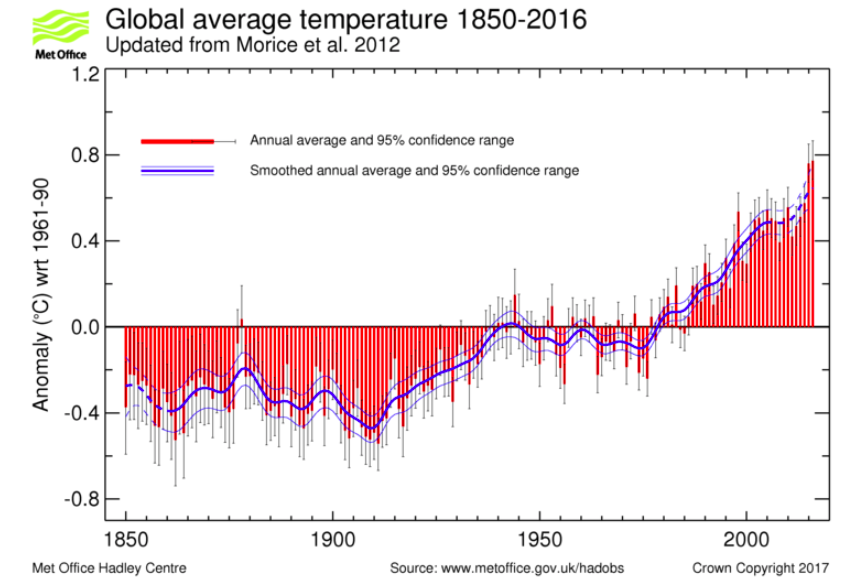
\includegraphics[scale=.30]{global.png}
\end{figure} 

\subsection{Loading the Data into R}
For our purpose, we are not interested in the spatial distribution, so we only use the \textit{Global Mean}.\\
Loading the data into R:
\begin{verbatim}
library(curl)
tmpf <- tempfile()
curl_download(url, tmpf)
gtemp <- read.table(tmpf)[, 1:2]
temp = gtemp$V2[1:2004]
\end{verbatim}
\indent We only use the first two columns: \textit{time and monthly global mean}. We pick the first 2004 observations, which is monthly data from $1850 \sim 2016$, so that the data has complete periods.\par
The time series of $temp$ is shown below:
\begin{figure}[H]
\centering
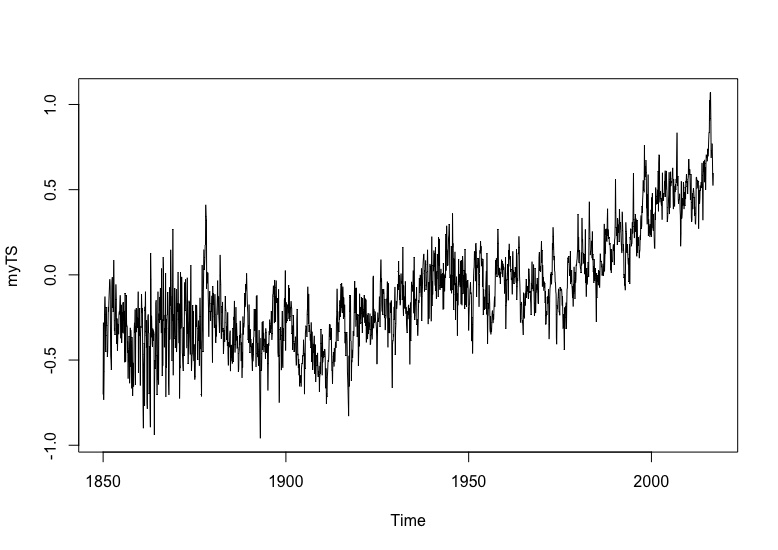
\includegraphics[scale=.45]{temp.png}
\end{figure}

\section{Dealing with the time series}

\subsection{Decompose}
The first thing we might want to do is to wipe out the seasonal component. There're many approaches to do it in R. We choose to use the $decompose()$ provided by $\{stats\}$. Looking at the time series, we think a additive model should be appropriate. \par
We can quickly checked that multiplicative model is not appropriate:
\begin{figure}[H]
\centering
\caption{multiplcative model: original ts, seasonal component, time trend, residuals}
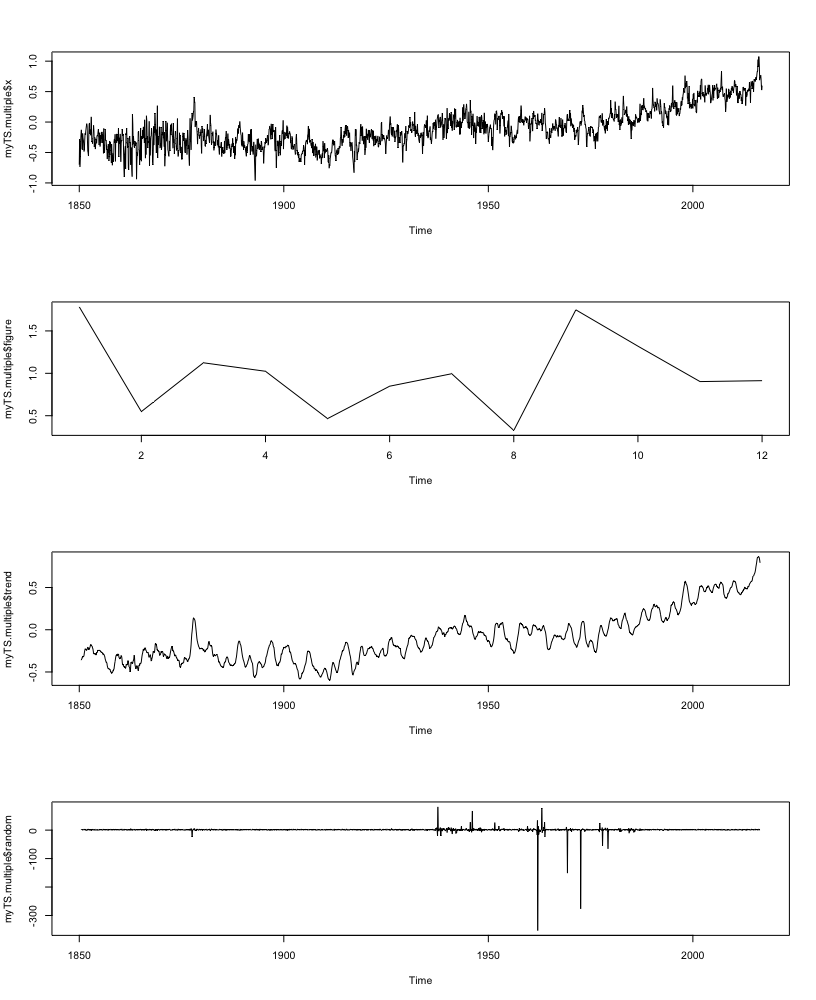
\includegraphics[scale=.40]{component2.png}
\end{figure}
Obviously the random term is not easy to be modelled.\par
Therefore, decompose the time series with additive method in the following code:
\begin{verbatim}
library(TSA)
myTS = ts(as.numeric(temp), start = c(1850, 1), frequency = 12)
myTS.additive = decompose(myTS)
myTS.adjusted = myTS.additive$x - myTS.additive$seasonal
\end{verbatim}
\indent The $myTS.adjusted$ now is free of seasonal components. The following graph illustrate the components.
\begin{figure}[H]
\centering
\caption{additive model: seasonal component, adjusted series}
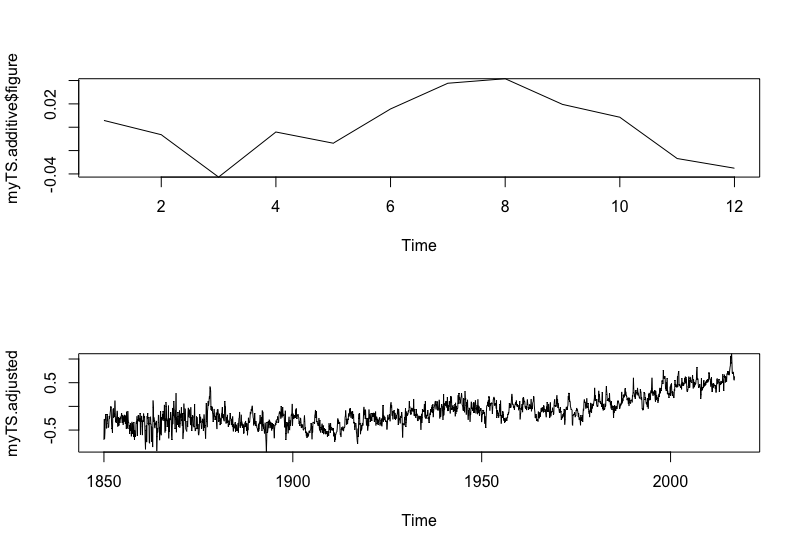
\includegraphics[scale=.50]{component.png}
\end{figure}
\indent Obviously, the time seires is not stationary. For simplicity, use \textit{diff()}.
\begin{verbatim}
dtemp = diff(myTS.adjusted)

> adf.test(dtemp)

	Augmented Dickey-Fuller Test

data:  dtemp
Dickey-Fuller = -16.175, Lag order = 12, p-value = 0.01
alternative hypothesis: stationary
\end{verbatim}
\indent So we can convince ourself that the time series $dtemp$ is stationary.

\subsection{Build a \textit{ARMA(p, q)} for \textit{dtemp}}
For simplicity, we use $auto.arima()$ from $\{forecast\}$ to judge the order.
\begin{verbatim}
library(forecast)
> auto.arima(dtemp> auto.arima(dtemp)
Series: dtemp 
ARIMA(2,0,4)(2,0,1)[12] with non-zero mean 

Coefficients:
         ar1     ar2      ma1      ma2     ma3     ma4    sar1    sar2     sma1   mean
      0.5041  0.3585  -1.0458  -0.1600  0.1362  0.0780  0.7619  0.0779  -0.7884  5e-04
s.e.  0.2431  0.2142   0.2423   0.3481  0.1082  0.0257  0.0926  0.0248   0.0910  2e-04

sigma^2 estimated as 0.01428:  log likelihood=1417.03
AIC=-2812.05   AICc=-2811.92   BIC=-2750.43

# first find the possible orders might be arma(2, 1) or arma(2, 4)

arma21.dtemp = arima(dtemp, c(2, 0, 1))
arma24.dtemp = arima(dtemp, c(2, 0, 4))

# next examine the two models' residuals

> auto.arima(arma21.dtemp$residuals)
Series: arma21.dtemp$residuals 
ARIMA(2,0,3)(2,0,1)[12] with zero mean     

Coefficients:
         ar1      ar2      ma1     ma2     ma3    sar1    sar2     sma1
      1.5859  -0.6762  -1.6089  0.6706  0.0506  0.7454  0.0748  -0.7785
s.e.  0.1156   0.1065   0.1169  0.1264  0.0297  0.1209  0.0258   0.1181

sigma^2 estimated as 0.01429:  log likelihood=1415.92
AIC=-2813.83   AICc=-2813.74   BIC=-2763.41

> auto.arima(arma24.dtemp$residuals)
Series: arma24.dtemp$residuals 
ARIMA(0,0,0) with zero mean     

sigma^2 estimated as 0.01435:  log likelihood=1408.31
AIC=-2814.63   AICc=-2814.62   BIC=-2809.02
\end{verbatim}
\indent Therefore it should be appropriate to choose \textit{arma(2, 4)} for series $dtemp$.

\begin{verbatim}
my.arma = arma24.dtemp

> my.arma

Call:
arima(x = dtemp, order = c(2, 0, 4))

Coefficients:
         ar1     ar2      ma1      ma2     ma3     ma4  intercept
      0.5204  0.3247  -1.0536  -0.1269  0.1168  0.0755      5e-04
s.e.  0.2733  0.2356   0.2727   0.3828  0.1117  0.0265      2e-04

sigma^2 estimated as 0.01435:  log likelihood = 1407.67,  aic = -2801.34

res = my.arma$residuals

> Box.test(res, type = 'Ljung-Box')

	Box-Ljung test

data:  res
X-squared = 0.0058853, df = 1, p-value = 0.9388
\end{verbatim}

\indent The $ARMA(2, 4)$ success in making the arma residual independent. 


\subsection{GARCH}
One can be pretty satisfied with the results right now. Yet Looking at the plot of arma residual:
\begin{figure}[H]
\centering
\caption{arma residual}
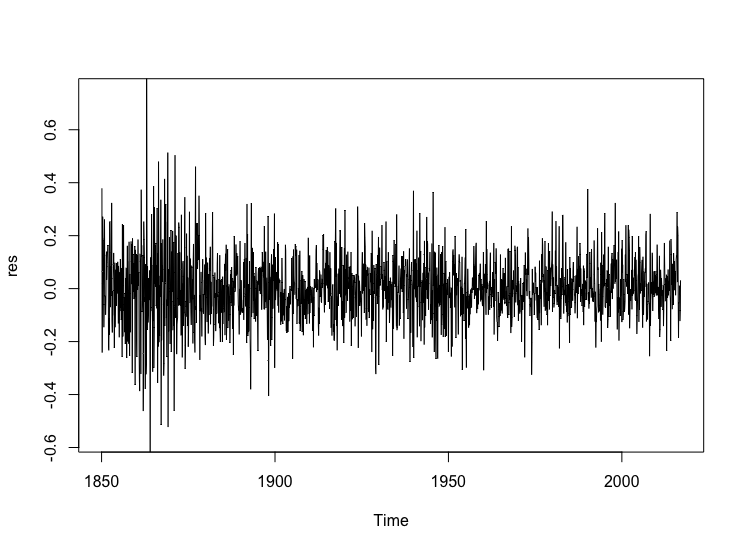
\includegraphics[scale=.60]{armares.png}
\end{figure}

\indent It makes us wondering if it has $ARCH$ effect. Using $arch.test$ from $\{aTSA\}$ to perform the $LM-Test$:
\begin{verbatim}
library(aTSA)
> arch.test(my.arma)
ARCH heteroscedasticity test for residuals 
alternative: heteroscedastic 

Portmanteau-Q test: 
     order    PQ p.value
[1,]     4  99.4       0
[2,]     8 116.9       0
[3,]    12 411.5       0
[4,]    16 475.6       0
[5,]    20 495.9       0
[6,]    24 755.8       0
Lagrange-Multiplier test: 
     order   LM p.value
[1,]     4 1418       0
[2,]     8  697       0
[3,]    12  418       0
[4,]    16  212       0
[5,]    20  168       0
[6,]    24  137       0
\end{verbatim}

\begin{figure}[H]
\centering
\caption{arma residual}
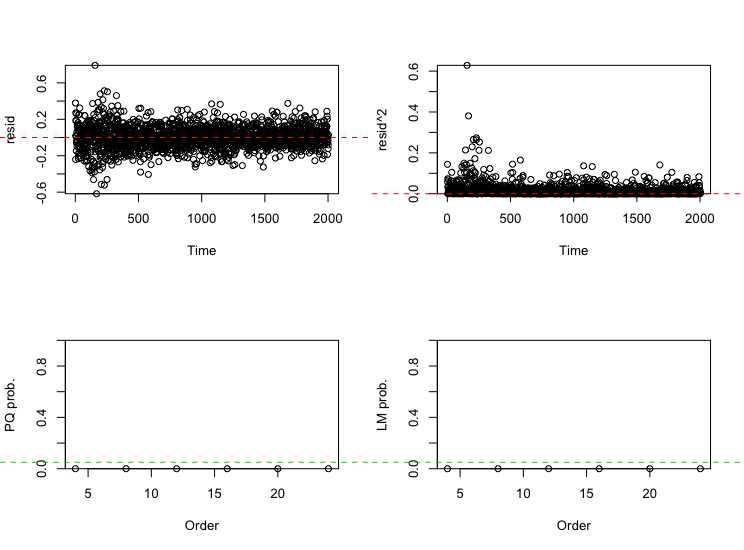
\includegraphics[scale=.50]{hetero.png}
\end{figure}



\indent It supports our doubt. Therefore we have the motive to build a $GARCH$ model. We decide to use the package $rugarch$.\par
\begin{equation*}
	\sigma_t^2 = (w + \sum_{j = 1}^m \zeta_j v_{jt}) + \sum_{j = 1}^q \alpha_j \varepsilon_{t-j}^2 + \sum_{j = 1}^p \beta_j \sigma_{t-j}^2
\end{equation*} 
\indent So we wrote a function:
\begin{verbatim}
library(rugarch)
my_sGARCH_test <- function(p, q, m, n, ts.data = res)
{
	# I use include.mean = FALSE after trying TRUE
	# to find out insignificance
    myspec=ugarchspec(variance.model = list(model = "sGARCH", garchOrder = c(p, q)), 
    	mean.model = list(armaOrder = c(m, n), include.mean = FALSE), 
    	distribution.model = "norm")
    myfit=ugarchfit(myspec,data=ts.data, solver="solnp")
    return(myfit)  
}
\end{verbatim}
\indent After trying a few times from $(1, 0), (0, 0, 0)$ to $(5, 5), (4, 0, 4)$, \textit{GARCH(1 ,1), ARIMA(2, 0, 3)} is the most satisfying model. Here we realize that using GARCH model, the order of ARIMA might changes.
\begin{verbatim}
fit1 = my_sGARCH_test(1, 1, 2, 3, dtemp)

> fit1

*---------------------------------*
*          GARCH Model Fit        *
*---------------------------------*

Conditional Variance Dynamics 	
-----------------------------------
GARCH Model	: sGARCH(1,1)
Mean Model	: ARFIMA(2,0,3)
Distribution	: norm 

Optimal Parameters
------------------------------------
        Estimate  Std. Error    t value Pr(>|t|)
ar1    -0.090935    0.015226    -5.9724 0.000000
ar2     0.754333    0.015069    50.0583 0.000000
ma1    -0.391906    0.007313   -53.5917 0.000000
ma2    -0.863257    0.000130 -6647.5909 0.000000
ma3     0.295634    0.007800    37.9010 0.000000
omega   0.000082    0.000034     2.3956 0.016595
alpha1  0.023026    0.003614     6.3706 0.000000
beta1   0.970594    0.004705   206.2925 0.000000

Robust Standard Errors:
        Estimate  Std. Error    t value Pr(>|t|)
ar1    -0.090935    0.017031    -5.3393 0.000000
ar2     0.754333    0.017312    43.5726 0.000000
ma1    -0.391906    0.002647  -148.0378 0.000000
ma2    -0.863257    0.000144 -6000.9074 0.000000
ma3     0.295634    0.002903   101.8443 0.000000
omega   0.000082    0.000036     2.2838 0.022382
alpha1  0.023026    0.003636     6.3329 0.000000
beta1   0.970594    0.003734   259.9413 0.000000

LogLikelihood : 1512.336 

Information Criteria
------------------------------------
                    
Akaike       -1.5021
Bayes        -1.4797
Shibata      -1.5021
Hannan-Quinn -1.4939

Weighted Ljung-Box Test on Standardized Residuals
------------------------------------
                         statistic p-value
Lag[1]                      0.3742  0.5407
Lag[2*(p+q)+(p+q)-1][14]    4.5219  1.0000
Lag[4*(p+q)+(p+q)-1][24]   13.5547  0.3236
d.o.f=5
H0 : No serial correlation

Weighted Ljung-Box Test on Standardized Squared Residuals
------------------------------------
                        statistic   p-value
Lag[1]                      31.06 2.506e-08
Lag[2*(p+q)+(p+q)-1][5]     37.84 1.904e-10
Lag[4*(p+q)+(p+q)-1][9]     51.28 4.433e-13
d.o.f=2

Weighted ARCH LM Tests
------------------------------------
            Statistic Shape Scale   P-Value
ARCH Lag[3]  0.004507 0.500 2.000 9.465e-01
ARCH Lag[5] 11.085543 1.440 1.667 3.565e-03
ARCH Lag[7] 20.592184 2.315 1.543 4.509e-05

Nyblom stability test
------------------------------------
Joint Statistic:  2.6294
Individual Statistics:              
ar1    0.25019
ar2    0.61592
ma1    0.19513
ma2    0.24162
ma3    0.07259
omega  0.10095
alpha1 0.42035
beta1  0.20019

Asymptotic Critical Values (10% 5% 1%)
Joint Statistic:     	 1.89 2.11 2.59
Individual Statistic:	 0.35 0.47 0.75

Sign Bias Test
------------------------------------
                   t-value      prob sig
Sign Bias           0.3363 7.367e-01    
Negative Sign Bias  3.6815 2.380e-04 ***
Positive Sign Bias  4.4421 9.396e-06 ***
Joint Effect       33.2983 2.786e-07 ***


Adjusted Pearson Goodness-of-Fit Test:
------------------------------------
  group statistic p-value(g-1)
1    20     57.32    1.019e-05
2    30     63.59    2.167e-04
3    40     85.01    2.883e-05
4    50    102.77    1.103e-05


Elapsed time : 0.365526
\end{verbatim}

\indent Substract the standardized(w.r.t. the variance model) residuals $z$, which is $z = \cfrac{residuals(fit)}{sigma(fit)}$.

\begin{verbatim}
z = residuals(fit1) / sigma(fit1)
plot.ts(z)
\end{verbatim}

\begin{figure}[H]
\centering
\caption{z}
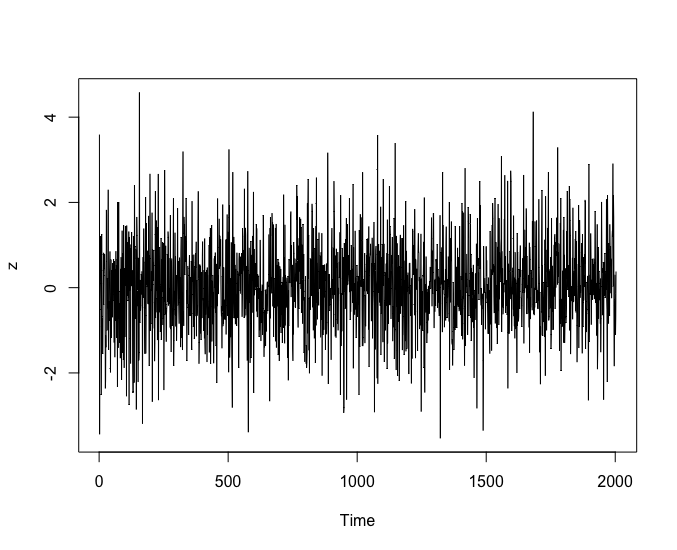
\includegraphics[scale=.40]{z.png}
\end{figure}

\indent We can compute the mean and variance of $z$:
\begin{verbatim}
> mean(z)
[1] 0.03181525
> var(z)
[1] 1.013866
> length(z)
[1] 2003
> plot.ts(rnorm(2003, 0.03181525, 1.013866))
\end{verbatim} 
\indent And then, just for fun, plot a normal sample series with the same parameters:

\begin{figure}[H]
\centering
\caption{simulation of using rnorm}
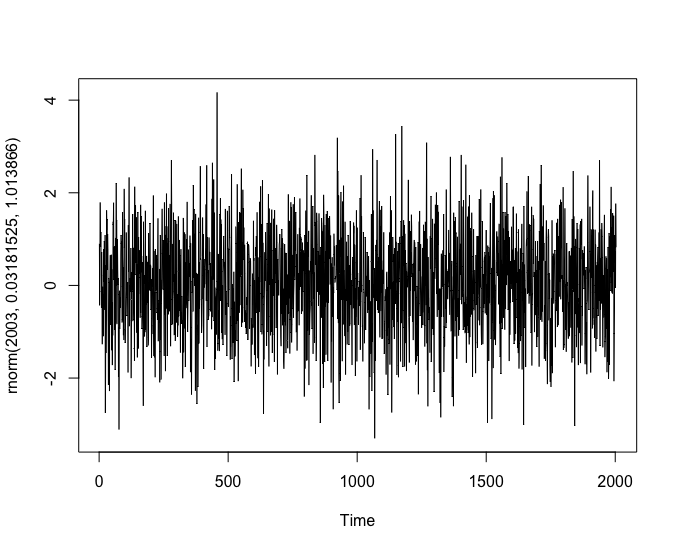
\includegraphics[scale=.40]{rnorm.png}
\end{figure}

\indent At least a human can't distinguish between them anymore. But what we most care about is whether standardized squared residuals can pass the $LM-Test$(substracting from the above long result):

\begin{verbatim}
Weighted ARCH LM Tests
------------------------------------
            Statistic Shape Scale   P-Value
ARCH Lag[3]  0.004507 0.500 2.000 9.465e-01
ARCH Lag[5] 11.085543 1.440 1.667 3.565e-03
ARCH Lag[7] 20.592184 2.315 1.543 4.509e-05
\end{verbatim}

We can see our model successfully wipes out ARCH effect at small lags, but fails at larger lags. This is the best `sGARCH' can give with respest to our data. Maybe we should try long memory models instead of \textit{diff()} at first.\par




\textbf{Graphical Diagnostics:}\par
The original series' acf is shown below(the difference of temperature):
\begin{figure}[H]
\centering
\caption{acf(dtemp)}
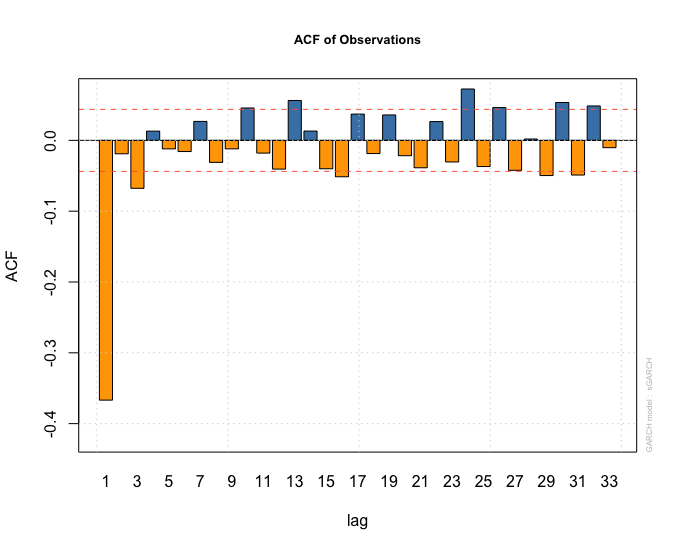
\includegraphics[scale=.60]{original_acf.png}
\end{figure}

The acf of standardized residuals:
\begin{figure}[H]
\centering
\caption{acf(z)}
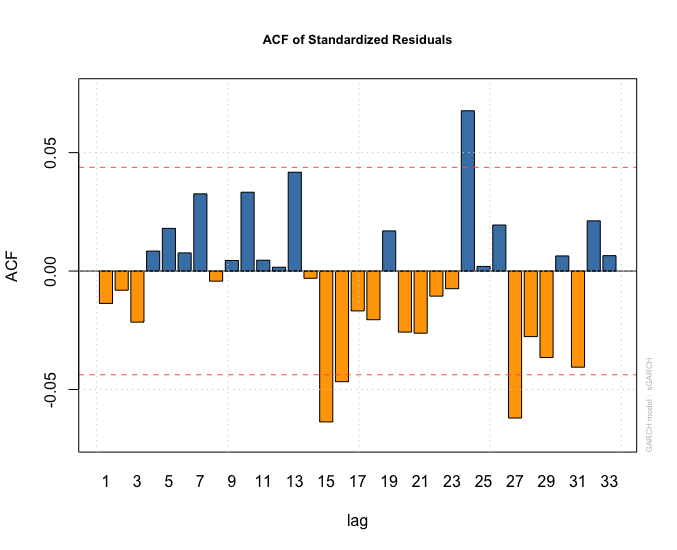
\includegraphics[scale=.60]{zacf.png}
\end{figure}
This is a prove that we should have used a long memory model.\par 


The \textit{Empirical Density of Standardized Residuals} compared to normal distribution:
\begin{figure}[H]
\centering
\caption{Empirical Density of Standardized Residuals}
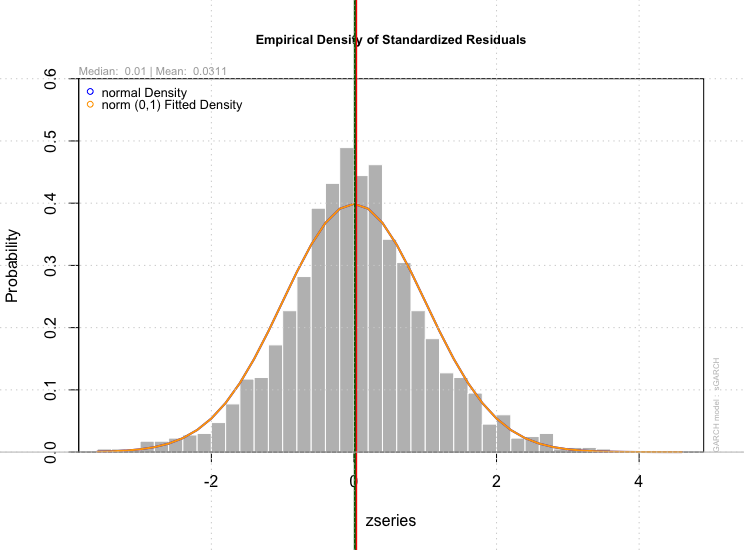
\includegraphics[scale=.60]{density.png}
\end{figure}
 
qqplot:
\begin{figure}[H]
\centering
\caption{qqplot of $z$}
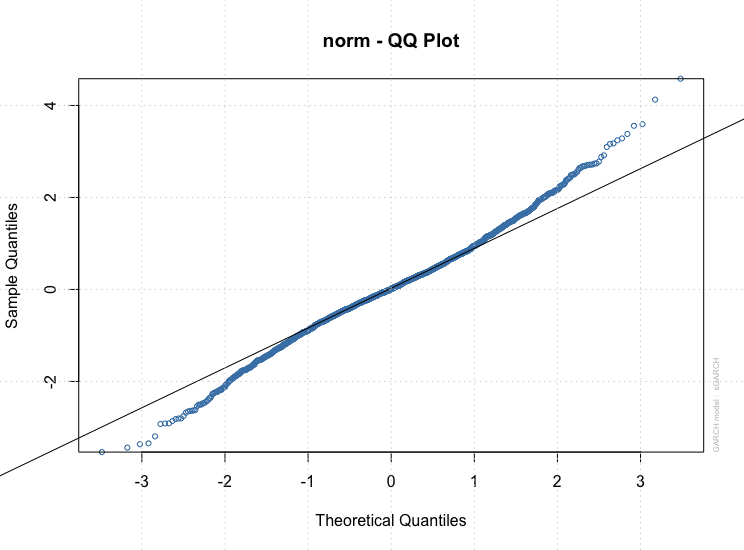
\includegraphics[scale=.60]{qqplot.png}
\end{figure}

\indent We can see that $z$ is skewed, which might be correlated with long lags' heterodasticity.\par

Series with 2 Conditional SD Superimposed:
\begin{figure}[H]
\centering
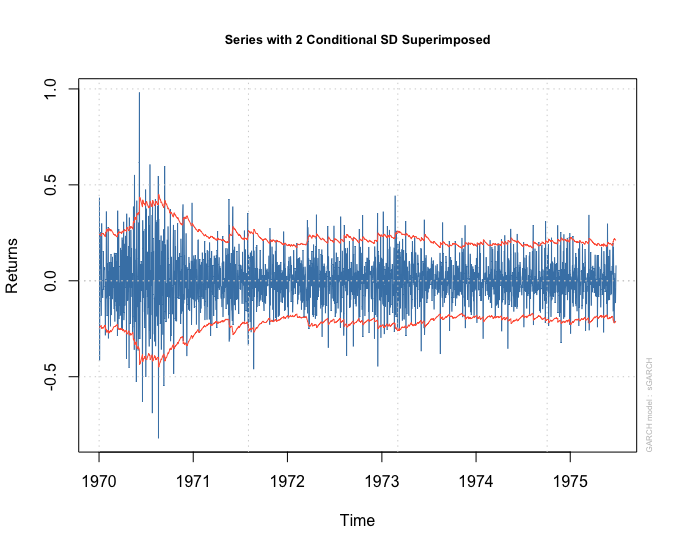
\includegraphics[scale=.60]{series_sd.png}
\end{figure}
\indent In this plot, we can find the reason that \textit{GARCH(1, 1)} can't completely wipe out heterodasticity, because there is a huge anomaly that can't be explained by an arma on variance.


\textbf{Forecast}

\begin{verbatim}
fore1 = ugarchforecast(fit1, n.ahead = 24)
fore.diff = as.numeric(fore1@forecast$seriesFor)
fore.sigma = as.numeric(fore1@forecast$sigmaFor)
ts.predict = temp[length(temp)] + cumsum(fore.diff)
ts.predict = ts.predict + myTS.additive$figure
ts.sigma = sqrt(cumsum(fore.sigma^2))
tsup.sigma = ts.predict + ts.sigma
tsdown.sigma = ts.predict - ts.sigma
plot(1:24, ts.predict, ylim=c(0,1.5), type = 'l', col = 'blue',
  xlab = "months", ylab = "temperature predict")
lines(1:24, tsup.sigma, type = 'l', col = 'red')
lines(1:24, tsdown.sigma, type = 'l', col = 'red')
\end{verbatim}

\begin{figure}[H]
\centering
\caption{forecast}
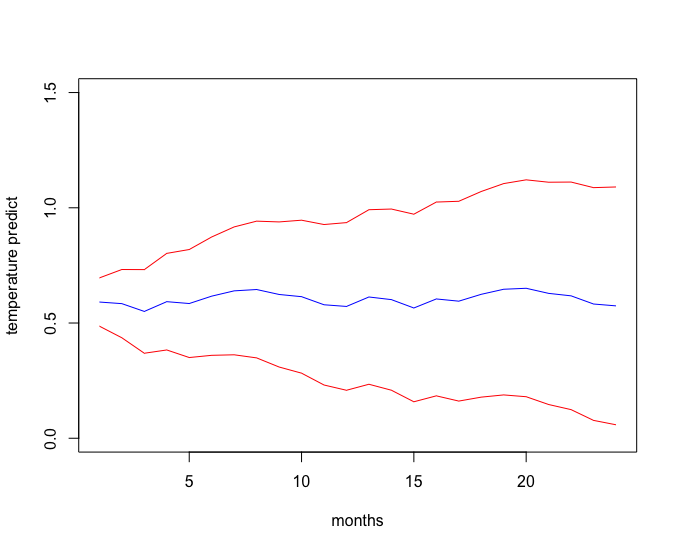
\includegraphics[scale=.60]{predict01.png}
\end{figure}


\textbf{Conclusion}: 'sGARCH' have improved the model in the intuitive sense and to some extent fix the heterodasticity. 




\end{document}